\documentclass{article}
\usepackage{graphicx, listings, xcolor}
\usepackage[letterpaper,top=1cm,bottom=2cm,left=1cm,right=1cm,marginparwidth=1cm]{geometry}

\lstset{
  basicstyle=\ttfamily\footnotesize,
  keywordstyle=\color{blue},
  stringstyle=\color{red},
  commentstyle=\color{gray},
  breaklines=true,
  showstringspaces=false,
  backgroundcolor=\color{gray!10}
}

\title{CISC866 Lab Report}
\author{Like Wang}

\begin{document}

\maketitle

\section{Encryption Mode: ECB vs. CBC}

\subsection{Display both encrypted image files}

\textit{Note: I chose to use the following method to get rid of the header issue:}
\begin{lstlisting}[language=Python]
    $ head -c 54 original1.bmp > header
    $ tail -c +55 encrypted1.bmp > body
    $ cat header body > new1.bmp
\end{lstlisting}
\textbf{Encryption command for ECB mode} (Note: iv not used by this cipher):
\begin{lstlisting}[language=Python]
$ openssl enc -aes-128-ecb -e -in pic_original1.bmp -out pic_1_ecb_enc.bmp -K 00112233445566778889aabbccddeeff
\end{lstlisting}
Picture look like this:\\
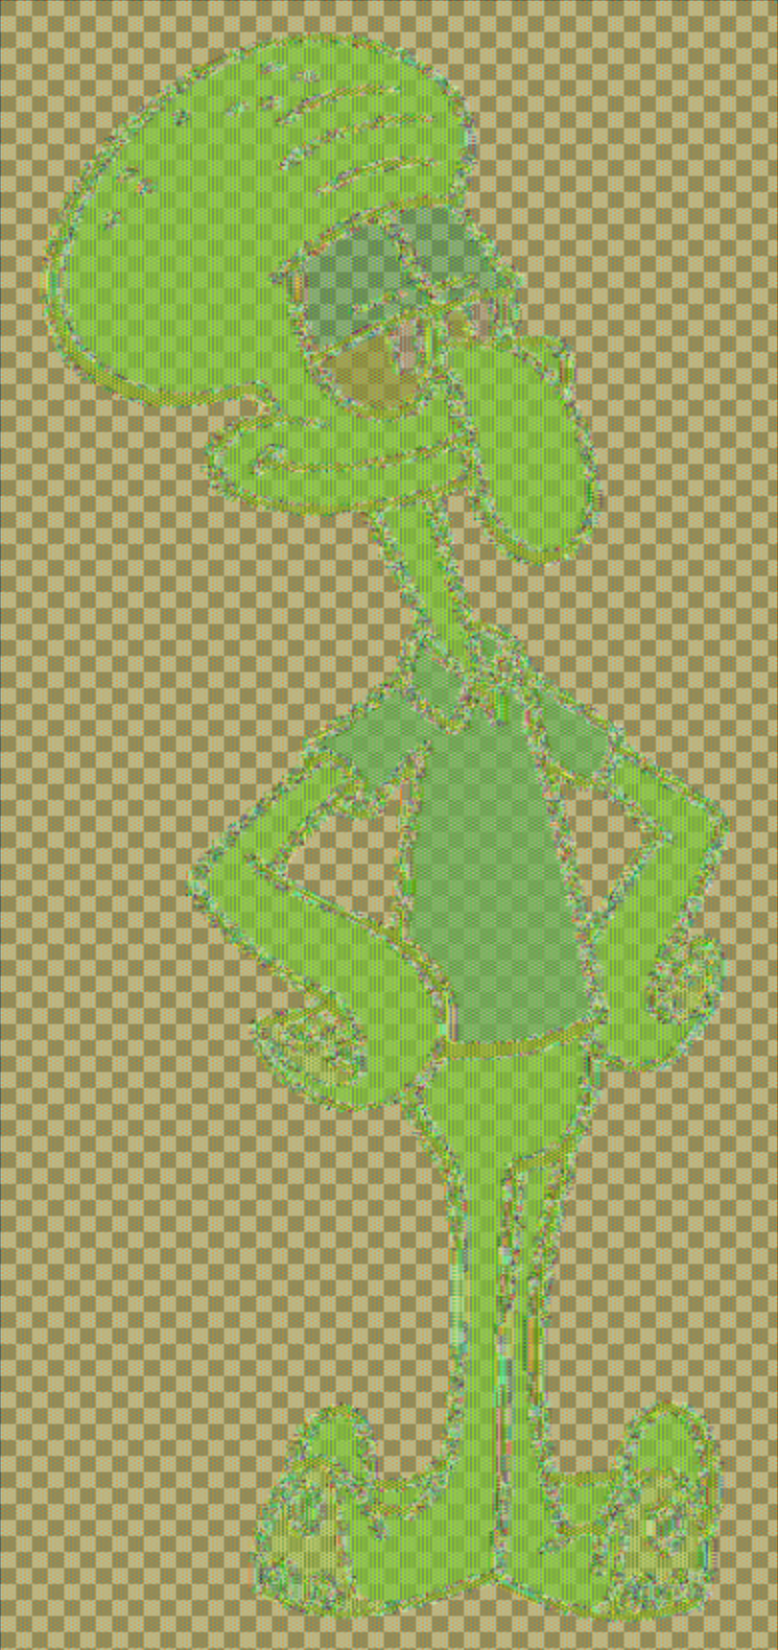
\includegraphics[height=5cm]{images/pic_1_ecb.png}

\textbf{Encryption command for CBC mode}:
\begin{lstlisting}[language=Python]
$ openssl enc -aes-128-cbc -e -in pic_original1.bmp -out pic_1_cbc_enc.bmp -K 00112233445566778889aabbccddeeff -iv 0102030405060708090a0b0c0d0e0f10
\end{lstlisting}
Picture look like this:\\
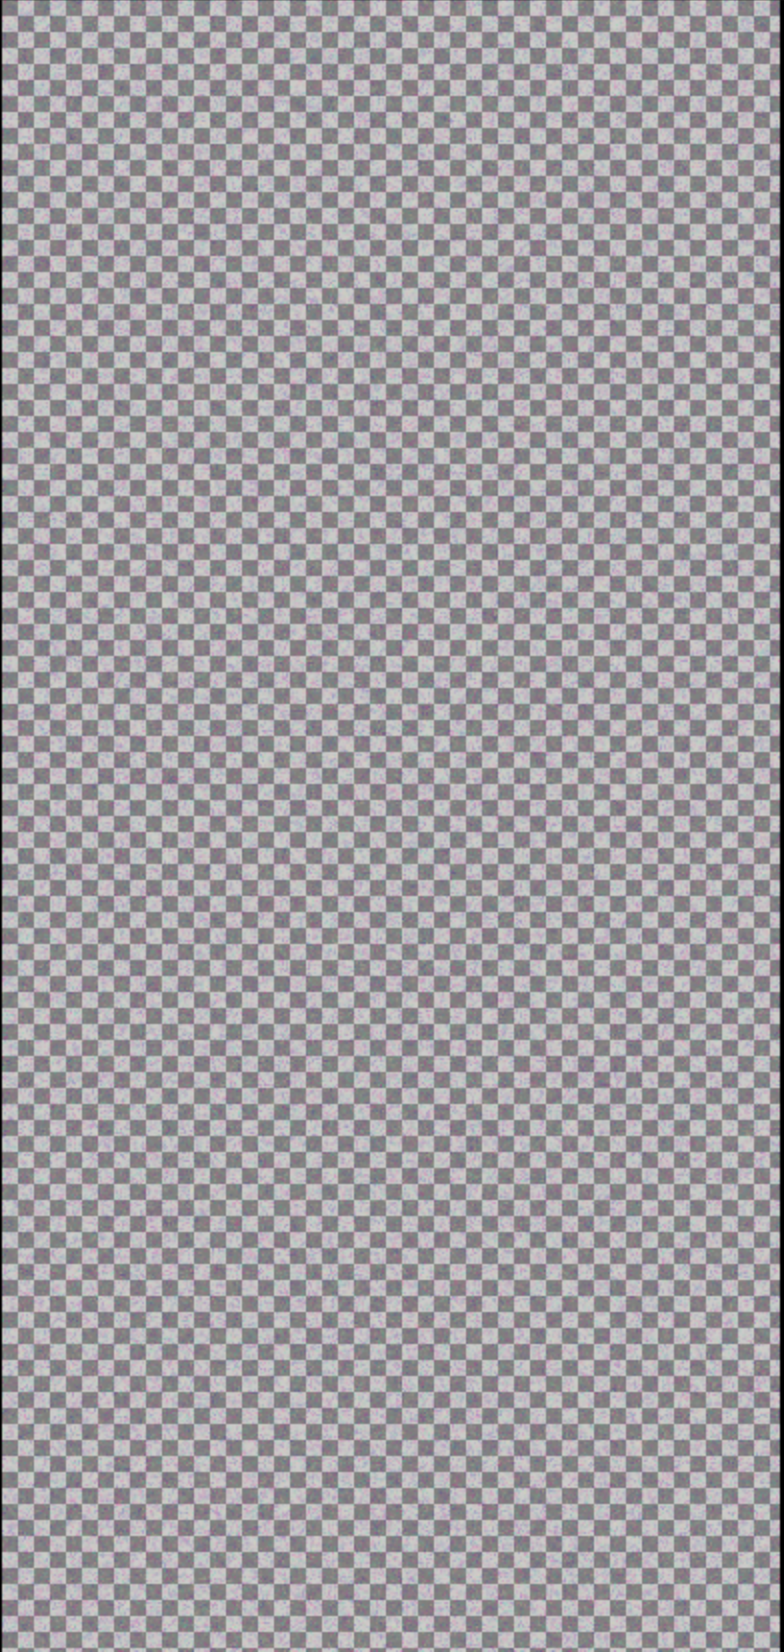
\includegraphics[height=5cm]{images/pic_1_cbc.png}

\subsection{Explain my observations}
From the two pictures above, we can see that the ECB mode encrypted image still retains some recognizable patterns from the original image, while the CBC mode encrypted image appears more random and does not reveal any discernible patterns. This is because ECB mode encrypts identical plaintext blocks into identical ciphertext blocks, making it vulnerable to pattern analysis. In contrast, CBC mode uses an initialization vector (IV) and chains the encryption of each block to the previous one, which helps to obscure patterns in the plaintext.

\end{document}